\documentclass[tikz]{standalone}

\usepackage{amsmath}
\usepackage{math}
\usepackage{color-scheme}

% colors
\colorlet{light}{color2!5!white}
\colorlet{dark}{color2!50!white}

% block fill colors
\colorlet{colorFun}{light}
\colorlet{colorNet}{light}
\colorlet{colorAlg}{light}
\colorlet{colorLMI}{light}
\colorlet{colorRho}{light}

\usetikzlibrary{calc,positioning}

\renewcommand{\emph}[1]{\textcolor{color1}{\textbf{#1}}}

\def\x{7.4mm}
\def\y{4.3cm}

\begin{document}

\begin{tikzpicture}[every node/.style={draw,rounded corners,thick,inner sep=2mm,align=center},
  every path/.style={->,very thick,>=latex,rounded corners}]

  \node (analysis) [minimum height=\y,text width=2cm,fill=colorLMI] {\textbf{Automated analysis}\\[2mm] (cvx opt problem)};

  \node (performance) [minimum height=\y,right=\x of analysis,text width=2.3cm,fill=colorRho] {\textbf{Performance bound}};
  
  \node (algorithm) [left=\x of analysis.south west,anchor=south east,text width=3.56cm,fill=colorAlg] {\textbf{Algorithm}\\[2mm] \centering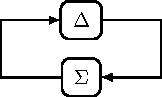
\includegraphics[scale=0.7]{sys-simple}};

  \node (functions) [left=\x of analysis.north west,anchor=north east,text width=4cm,fill=colorFun] {\textbf{Optimization problem}\\[2mm] $\begin{aligned} \minimize &\quad f(x) \\ \textrm{subject to} &\quad x\in X \end{aligned}$};

  \draw (algorithm) -- (algorithm.east -| analysis.west);
  \draw (functions.east) -- (functions.east -| analysis.west);
  \draw (analysis) -- (performance);
\end{tikzpicture}

\end{document}
